\section{Informationskrav}\label{sec:informations-krav}
\todo{introduktion og Unified process}

\subsection{Domænemodel}\label{Domainmodel}
Domænemodellen beskriver de relationer klasserne har til hinanden, samt hvilke attributter de indeholder. Her laves domænemodellen ud fra Kandidatklasserne og arkitektur principper.

\begin{figure}[H]
    \centering
    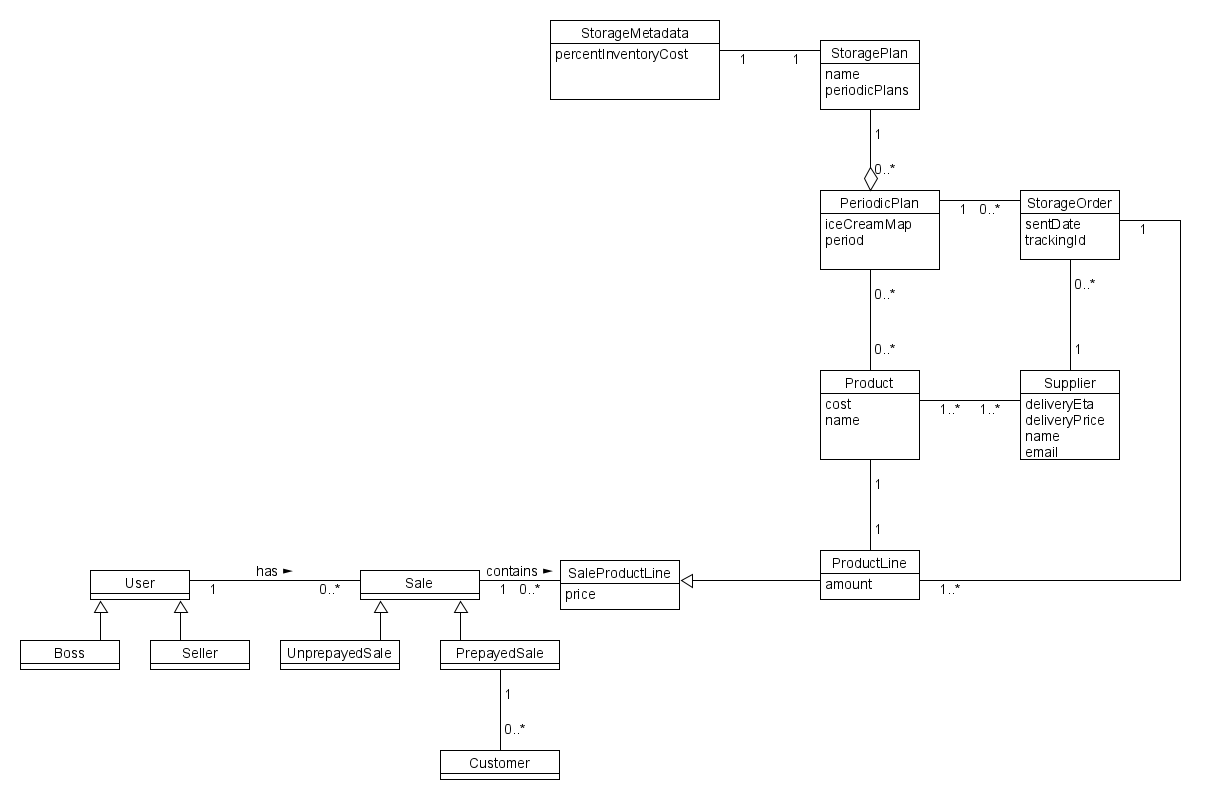
\includegraphics[width=0.9\textwidth]{figures/krav/domain_model_1.png}
    \caption{Domænemodel 1}
    \label{fig:domain_model}
\end{figure}

Domænemodellen som ses ovenfor viser hvordan klasserne er repræsenteret og hvilke relationer de har til hinanden. SeasonalPlan er planen, som beskriver hvordan lageret skal være hos Hjem-IS. Sæsonplanen for lagerbeholdningen bestemmes af hvilke produkter der er på lager, og hvor meget der bliver solgt. Ud fra dette kan der laves en bestilling (StorageOrder), som indeholder informationer om hvilke produkter der skal bestilles, hvilken Supplier de skal bestilles fra. Disse bestillingsplaner bestemmer sæsonplanen.
For at kunne gennemføre Use Casen er det ikke nødvendigt endnu at tage højde for Sales og Users, da det kun er Products og Storage ændringer der er relevante. 

\begin{figure}[H]
    \centering
    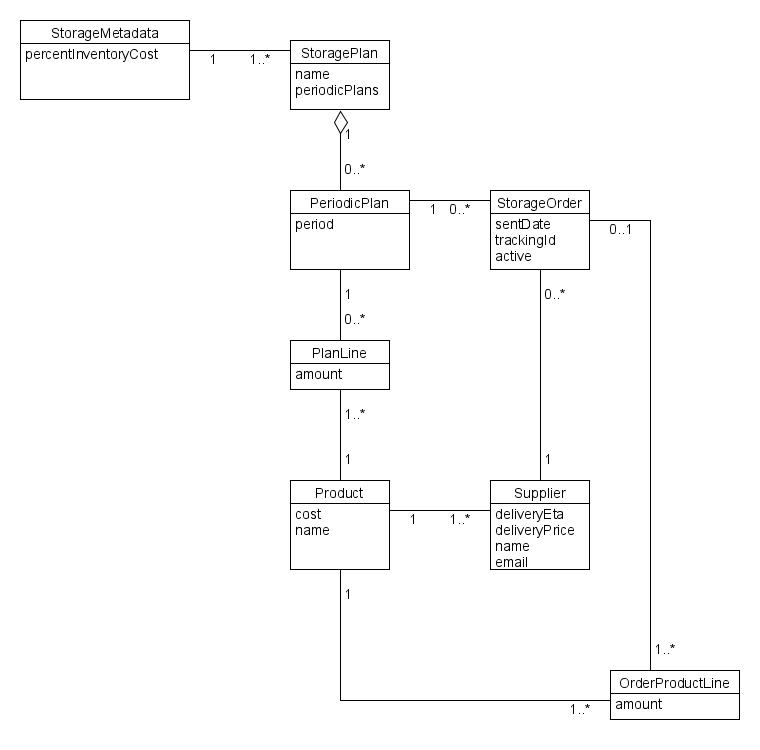
\includegraphics[width=0.9\textwidth]{figures/krav/domain_model_2.png}
    \caption{Domænemodel 2}
    \label{fig:domain_model_2}
\end{figure}

Domænemodellen ovenfor forholder sig kun til de relevante klasser for at kunne gennemføre Use Casen Automatisk Lagerstyring. Det er ud fra denne at databasen vil blive designet.

\subsection{Database}
Nu hvor domænemodellen er på plads kan der nu også udvikles en relational model af databasen. Der vil først tages udgangspunkt i at mappe hver klasse til en tabel, hvor der tages højde for klassenavn og attributter.
Da der ingen nedarvning er mellem nogen af klasserne, er det ikke relevant at tænke i pull-up og pull-down. Hver klasse får derfor sin egen tabel.
Dernæst skal associationerne laves ud fra om der er tale om 1-til-1, 1-til-mange eller mange-til-mange relationer. 

\begin{figure}[H]
    \centering
    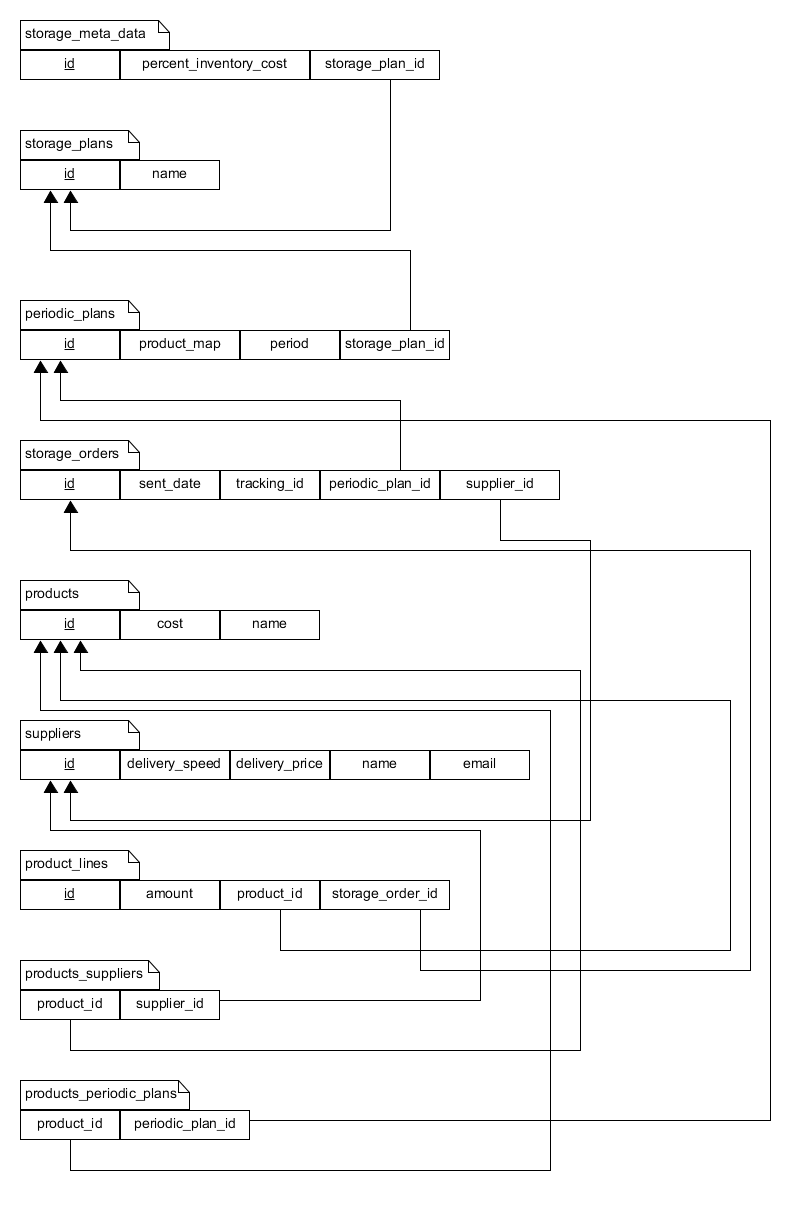
\includegraphics[width=0.9\textwidth]{figures/krav/relation_model_0th_normalization.png}
    \caption{Relationsmodel før normalisering}
    \label{fig:relational_model_0}
\end{figure}

Reglerne for de forskellige relationer og hvordan de skal forbindes er fulgt under udviklingen af den relationelle model, hvilket bl.a. kan ses på 'product\_supplier' tabellen. Denne forbinder en mange-til-mange association mellem Product og Supplier. 
Nu hvor tabellen er lavet, kan den normaliseres.

Efter at have kigget tabellen igennem kan det ses at 1NF er opfyldt da alle værdier er atomiske.
For at opfylde 2NF skal 1NF være opfyldt, og der skal ikke være nogle partial dependencies. Da der skal bruges en Map mellem 'products' og 'seasonal\_plans' laves der en ny tabel: 'seasonal\_plan\_product\_maps'. Denne vil også indeholde 'amount'.

\begin{figure}[H]
    \centering
    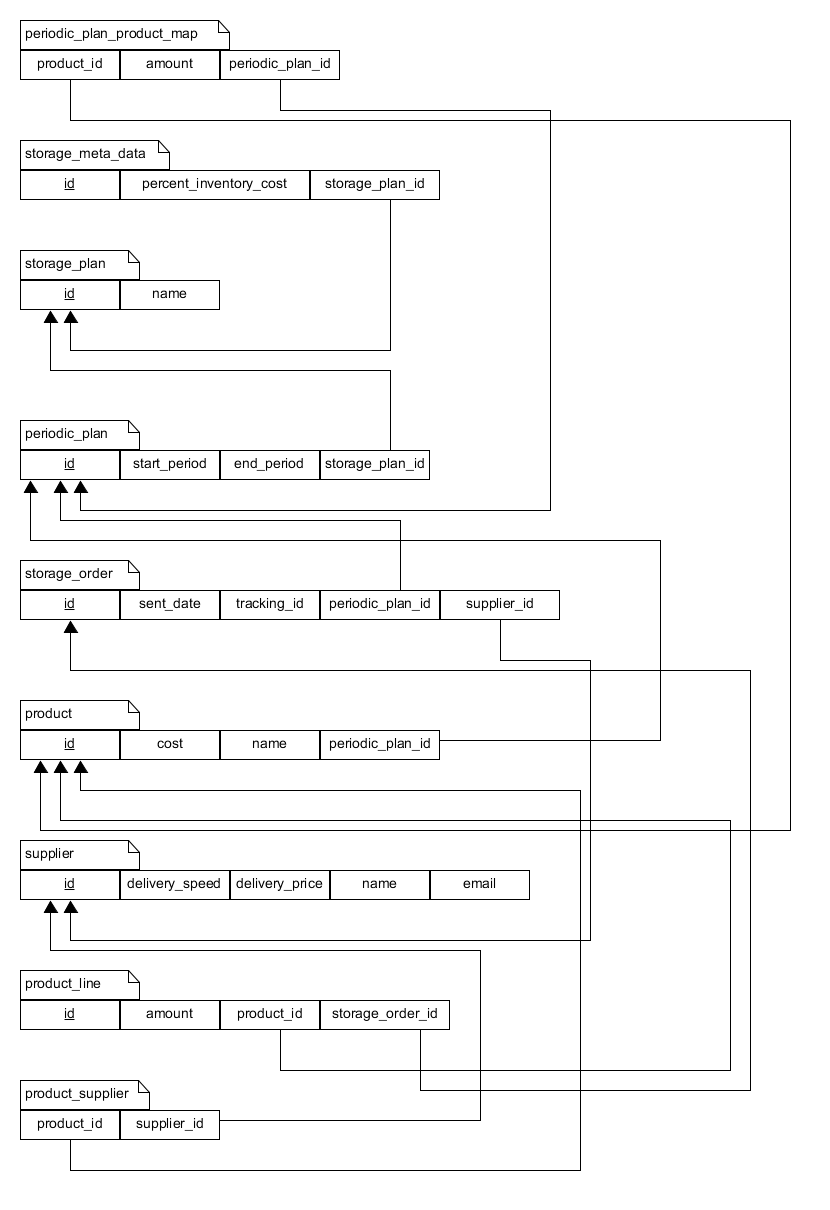
\includegraphics[width=0.9\textwidth]{figures/krav/relation_model_1th_normalization.png}
    \caption{Relationsmodel efter 2NF}
    \label{fig:relational_model_0}
\end{figure}

For at opfylde 3NF skal 2NF være opfyldt, og der må ikke være nogle transitive afhængigheder. Det minder meget om kravet til 2NF, og det kan konkluderes at der ingen transitive afhængigheder er.
For at opfylde BCNF kræves det at 3NF er opfyldt og at samtlige determinanter er kandidatnøgler. De determinanter, der er I den relationelle model er samtlige attributter med 'id' og '...\_id' på nær 'tracking\_id'. 'tracking\_id' sent\_date på varen. Der er derfor ingen afhængighed. 

Det kan nu konkluderes at den relationelle model er på BCNF og kan udvikles i Microsoft SQL.
